\documentclass[11pt,a4paper]{article}
\usepackage[danish]{babel}
\usepackage[T1]{fontenc}
\usepackage[utf8]{inputenc}
\usepackage{icomma}
\usepackage{amsmath, amssymb, mathtools}
\usepackage{booktabs, enumitem}
\usepackage{graphicx}
\usepackage{xcolor}
\usepackage[most]{tcolorbox}
\tcbuselibrary{skins, breakable}
\usepackage{tikz}
\usetikzlibrary{calc, arrows.meta}
\usepackage[hidelinks]{hyperref}
\usepackage[capitalise]{cleveref}
\usepackage{geometry}
\geometry{a4paper, margin=2.3cm}
\usepackage{parskip}
\usepackage{multicol}
\usepackage{titlesec}
\usepackage{fancyhdr}

% --- hus-system (fra gxu-funktioner-og-ligninger.tex) ------------------------
\definecolor{gxu-paper}{HTML}{F7F9FB}
\definecolor{gxu-ink}{HTML}{1A1F2B}
\definecolor{gxu-inksoft}{HTML}{4A5568}
\definecolor{gxu-accent}{HTML}{58C4DD}
\definecolor{gxu-purple}{HTML}{7C5CFC}

\pagestyle{fancy}
\fancyhf{}
\fancyhead[L]{\sffamily\small\color{gxu-inksoft}GXU -- Matematik}
\fancyhead[R]{\sffamily\small\color{gxu-inksoft}Træningsopgavesæt 5}
\fancyfoot[C]{\sffamily\small\color{gxu-inksoft}\thepage}

\renewcommand{\headrulewidth}{0.0pt}

\makeatletter
\newcommand{\eq}[2]{\begin{equation}#2\tag{#1}\end{equation}}
\makeatother
\newcommand{\note}[1]{{\small\color{gxu-inksoft}\textit{#1}}\par\vspace{4pt}}

% ── farver ──────────────────────────────────────────────────────────────────
\definecolor{accent}{HTML}{58C4DD}
\definecolor{accentdark}{HTML}{2A8FB8}
\definecolor{ink}{HTML}{1A1F2B}
\definecolor{inksoft}{HTML}{4A5568}
\definecolor{rule}{HTML}{D6D9DD}
\definecolor{boxbg}{HTML}{F7F9FB}
\definecolor{boxframe}{HTML}{CBD5E0}
\definecolor{kulred}{HTML}{C0392B}
\definecolor{kulblaa}{HTML}{2C5FA8}
\definecolor{kulgron}{HTML}{2E7D4F}
\definecolor{graysk}{HTML}{E2E6EA}

% ── boks-stil ───────────────────────────────────────────────────────────────
\newtcolorbox{opgavebox}{
  enhanced, breakable,
  colback=boxbg, colframe=boxframe,
  boxrule=0.4pt, arc=2pt, left=4pt, right=4pt, top=3pt, bottom=3pt,
  before skip=8pt, after skip=8pt
}
\newtcolorbox{regelbox}{
  enhanced, breakable,
  colback=boxbg, colframe=accent,
  boxrule=0.6pt, arc=2pt, left=6pt, right=6pt, top=4pt, bottom=4pt,
  before skip=8pt, after skip=8pt
}

% ── titel-stil ──────────────────────────────────────────────────────────────
\titleformat{\section}{\Large\bfseries\color{accent}}{\thesection}{0.6em}{}
\titleformat{\subsection}{\large\bfseries\color{accent}}{\thesubsection}{0.6em}{}
\titlespacing*{\section}{0pt}{1.1em}{0.5em}
\titlespacing*{\subsection}{0pt}{0.8em}{0.4em}

% ── makroer ─────────────────────────────────────────────────────────────────
% Kompetence-chips (samme som gxu-funktioner-og-ligninger.tex)
\newcommand{\kompetence}[1]{%
  \tcbox[on line, colback=gxu-accent!15, colframe=gxu-accent, boxrule=0.4pt,
         arc=10pt, left=6pt, right=6pt, top=3pt, bottom=3pt, boxsep=0pt,
         fontupper=\sffamily\small]{#1}\hspace{5pt}%
}
\newcommand{\kompetencer}[1]{\kompetence{#1}}

% Retvinklet trekant med vinkel A i højre hjørne.
% \trek{b}{a}{vinkelmærke}{b-etiket}{c-etiket}{a-etiket}{skala}
\newcommand{\trek}[7]{%
\begin{tikzpicture}[scale=#7, line cap=round, line join=round]
  \coordinate (B) at (0,0);
  \coordinate (A) at (#1,0);
  \coordinate (C) at (0,#2);
  \draw[thick] (B) -- (A) -- (C) -- cycle;
  \draw[thick] ($(B)+(0.25,0)$) -- ($(B)+(0.25,0.25)$) -- ($(B)+(0,0.25)$);
  \pgfmathsetmacro{\vinkelSlut}{180 - atan2(#2,#1)}
  \draw[thick] ($(A)+(180:0.55)$) arc[start angle=180, end angle=\vinkelSlut, radius=0.55];
  \pgfmathsetmacro{\vinkelMid}{(180 + \vinkelSlut)/2}
  \node[anchor=west] at ($(A)+(\vinkelMid:0.95)$) {\small #3};
  \node[below] at ($ (B)!0.5!(A) $) {#4};
  \node[right] at ($ (A)!0.5!(C) $) {#5};
  \node[left]  at ($ (B)!0.5!(C) $) {#6};
\end{tikzpicture}%
}

% Brøkstribe: n dele i alt, k dele farvet.
% \fraktionsstribe{n}{k}{skala}{etiket}
\newcommand{\fraktionsstribe}[4]{%
\begin{tikzpicture}[scale=#3, line cap=round]
  \fill[accent!55] (0,0) rectangle (#2,1);
  \foreach \i in {1,...,#1} \draw[thin, inksoft] (\i,0) -- (\i,1);
  \draw[thick] (0,0) rectangle (#1,1);
  \node[below, font=\small, text=inksoft] at (#1/2,-0.12) {#4};
\end{tikzpicture}%
}

% Terning med pips (1-6).
\newcommand{\die}[1]{%
\begin{tikzpicture}[scale=1.15,baseline=-0.6ex]
  \draw[thick, rounded corners=2pt, fill=boxbg] (0,0) rectangle (1,1);
  \ifcase#1\relax
  \or \fill[ink] (0.5,0.5) circle (0.085);
  \or \fill[ink] (0.28,0.72) circle (0.085); \fill[ink] (0.72,0.28) circle (0.085);
  \or \fill[ink] (0.28,0.72) circle (0.085); \fill[ink] (0.5,0.5) circle (0.085); \fill[ink] (0.72,0.28) circle (0.085);
  \or \fill[ink] (0.28,0.72) circle (0.085); \fill[ink] (0.72,0.72) circle (0.085);
       \fill[ink] (0.28,0.28) circle (0.085); \fill[ink] (0.72,0.28) circle (0.085);
  \or \fill[ink] (0.28,0.72) circle (0.085); \fill[ink] (0.72,0.72) circle (0.085);
       \fill[ink] (0.5,0.5) circle (0.085);
       \fill[ink] (0.28,0.28) circle (0.085); \fill[ink] (0.72,0.28) circle (0.085);
  \or \fill[ink] (0.28,0.72) circle (0.085); \fill[ink] (0.72,0.72) circle (0.085);
       \fill[ink] (0.28,0.5) circle (0.085); \fill[ink] (0.72,0.5) circle (0.085);
       \fill[ink] (0.28,0.28) circle (0.085); \fill[ink] (0.72,0.28) circle (0.085);
  \fi
\end{tikzpicture}%
}

% Krukke med kugler.
\newcommand{\krukke}{%
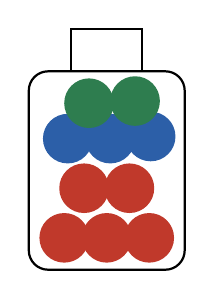
\begin{tikzpicture}[scale=0.9]
  \fill[kulred]  (-0.60,0.45) circle (0.35);
  \fill[kulred]  ( 0.00,0.45) circle (0.35);
  \fill[kulred]  ( 0.60,0.45) circle (0.35);
  \fill[kulred]  (-0.32,1.15) circle (0.35);
  \fill[kulred]  ( 0.32,1.15) circle (0.35);
  \fill[kulblaa] (-0.55,1.85) circle (0.35);
  \fill[kulblaa] ( 0.05,1.85) circle (0.35);
  \fill[kulblaa] ( 0.62,1.88) circle (0.35);
  \fill[kulgron] (-0.25,2.35) circle (0.35);
  \fill[kulgron] ( 0.40,2.38) circle (0.35);
  \draw[thick, rounded corners=7pt] (-1.10,0) rectangle (1.10,2.80);
  \draw[thick] (-0.50,2.80) -- (-0.50,3.40) -- (0.50,3.40) -- (0.50,2.80);
\end{tikzpicture}%
\qquad
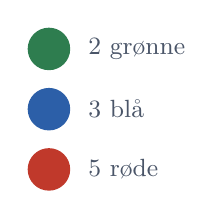
\begin{tikzpicture}[scale=0.9]
  \fill[kulred]  (0,0) circle (0.30);
  \fill[kulblaa] (0,0.85) circle (0.30);
  \fill[kulgron] (0,1.70) circle (0.30);
  \node[right, font=\small, text=inksoft] at (0.42,0)     {$5$ røde};
  \node[right, font=\small, text=inksoft] at (0.42,0.85)  {$3$ blå};
  \node[right, font=\small, text=inksoft] at (0.42,1.70) {$2$ grønne};
\end{tikzpicture}
}

% Kasse i skråprojektion.
% \kassefigur{l-tekst}{b-tekst}{h-tekst}{skala}
% Kasse i skraaprojektion, tegnet i skala: 12 cm -> 3,6 enheder (0,30 pr. enhed),
% 8 cm dybde -> forskydning (1,7;1,7), 5 cm hoejde -> 1,5 enheder.
\newcommand{\kassefigur}[4]{%
\begin{tikzpicture}[scale=#4, line cap=round, line join=round]
  % forside (12 x 5)
  \draw[thick] (0,0) -- (3.6,0) -- (3.6,1.5) -- (0,1.5) -- cycle;
  % hojre sideflade
  \draw[thick] (3.6,0) -- (5.3,1.7) -- (5.3,3.2) -- (3.6,1.5);
  % topflade
  \draw[thick] (0,1.5) -- (1.7,3.2) -- (5.3,3.2);
  % skjulte kanter
  \draw[thick, dashed] (0,0) -- (1.7,1.7);
  \draw[thick, dashed] (1.7,1.7) -- (5.3,1.7);
  \draw[thick, dashed] (1.7,1.7) -- (1.7,3.2);
  \node[below, font=\small, text=inksoft] at (1.8,0)      {#1};
  \node[below right, font=\small, text=inksoft, xshift=2pt, yshift=-1pt] at (4.45,0.85) {#2};
  \node[left,  font=\small, text=inksoft] at (0,0.75)     {#3};
\end{tikzpicture}%
}

% Cylinder i skråprojektion.
% \cylinderfigur{r-tekst}{h-tekst}{skala}
\newcommand{\cylinderfigur}[3]{%
\begin{tikzpicture}[scale=#3, line cap=round, line join=round]
  \draw[thick] (0,2.52) ellipse (1.05 and 0.30);
  \draw[thick] (-1.05,0) arc[start angle=180, end angle=360, x radius=1.05, y radius=0.30];
  \draw[thick, dashed] (1.05,0) arc[start angle=0, end angle=180, x radius=1.05, y radius=0.30];
  \draw[thick] (-1.05,0) -- (-1.05,2.52);
  \draw[thick] ( 1.05,0) -- ( 1.05,2.52);
  \draw[densely dashed, line width=0.5pt] (0,2.52) -- (1.05,2.52);
  \node[right, font=\small, text=inksoft] at (1.10,2.52) {#1};
  \draw[<->, line width=0.5pt, {Stealth[length=4pt]}-{Stealth[length=4pt]}] (-1.35,0) -- (-1.35,2.52);
  \node[left, font=\small, text=inksoft] at (-1.42,1.26) {#2};
\end{tikzpicture}%
}

\title{}
\author{}
\date{}

\begin{document}

\begin{center}
  {\Large\bfseries Træningsopgavesæt 5}\\[2pt]
  {\color{inksoft}\large Brøker, procent, sandsynlighed, trigonometri og geometri}\\[6pt]
  {\color{inksoft}\small Fra Omar og Karoline --- 18.~november 2026}
\end{center}

\vspace{6pt}
\hrule height 0.4pt
\vspace{10pt}

\noindent
Dette er et træningssæt med seks emner: brøker, procentregning, sandsynlighed,
trigonometri, 2D-geometri og 3D-geometri. Hvert emne starter med en kort regel
og et udregnet eksempel --- så kan du løse opgaverne på samme måde. Alle
facit ligger bagerst.

\vspace{4pt}
\noindent
{\small\color{inksoft}\textit{Sådan bruger du sættet: Læs reglen, kig på
eksemplet, og brug derefter samme metode på opgaverne. Skriv alle
mellemregninger ned --- det er der, pointen tænkes.}}

% ═════════════════════════════════════════════════════════════════════════════
\section{Brøker}
% ═════════════════════════════════════════════════════════════════════════════

\kompetence{Regning}\kompetence{Repræsentation}\kompetence{Problembehandling}

\noindent
En brøk fortæller, hvor stor en del ud af en helhed vi tager. Tælleren står
øverst, nævner nederst. $\tfrac{3}{4}$ betyder \emph{tre firedele}.

\subsection*{Regel 1 --- Brøk af en mængde}

\begin{regelbox}
\textbf{Regel:} Del tallet i så mange lige dele som nævneren siger, og tag så
mange dele som tælleren siger. Det kan du gøre med division: tal $\div$
nævner, og så ganger du med tælleren.
\end{regelbox}

\textbf{Eksempel: Hvad er $\tfrac{3}{4}$ af $60\,\text{kr}$?}

\begin{center}
\fraktionsstribe{4}{3}{0.85}{$3$ af $4$ dele}
\end{center}

\begin{align*}
  60 \div 4 &= 15 \qquad\text{(en del)}\\
  3 \cdot 15 &= 45 \qquad\text{(tre dele)}\\
  \tfrac{3}{4} \text{ af } 60\,\text{kr} &= 45\,\text{kr}
\end{align*}

\begin{opgavebox}
\textbf{Opgave 1.1} \quad Hvad er $\tfrac{2}{7}$ af $63$? \hfill
{\small\color{inksoft}(Hjælp: $63 \div 7 = 9$)}
\end{opgavebox}

\begin{opgavebox}
\textbf{Opgave 1.2} \quad En klasse har $32$ elever. $\tfrac{3}{8}$ af dem går
i svømmehal. Hvor mange elever går der?
\end{opgavebox}

\subsection*{Regel 2 --- Brøk, decimaltal og procent}

\begin{regelbox}
\textbf{Regel:} En brøk kan skrives som et decimaltal ved at dividere tæller
med nævner. Og et decimaltal kan skrives i procent ved at gange med $100$.
\end{regelbox}

\textbf{Eksempel: $\tfrac{3}{8}$ som decimaltal og procent}
\begin{align*}
  3 \div 8 &= 0{,}375\\
  0{,}375 \cdot 100 &= 37{,}5\,\%\\
  \text{Altså: } \tfrac{3}{8} &= 0{,}375 = 37{,}5\,\%
\end{align*}

\begin{opgavebox}
\textbf{Opgave 1.3} \quad Skriv $0{,}45$ som en brøk i mindste form.
\end{opgavebox}

\begin{opgavebox}
\textbf{Opgave 1.4} \quad Skriv $\tfrac{2}{5}$ som procent.
\end{opgavebox}

\subsection*{Regel 3 --- Sammenlign to brøker}

\begin{regelbox}
\textbf{Regel:} Find en fællesnævner --- et tal som begge nævnere går op i.
Forlæng begge brøker til den nævner, og sammenlign så tællerne. Den brøk
med størst tæller er størst.
\end{regelbox}

\textbf{Eksempel: Hvilken er størst, $\tfrac{3}{5}$ eller $\tfrac{5}{8}$?}
\begin{align*}
  \text{Fællesnævner for } 5 \text{ og } 8 \text{ er } 40.\\[2pt]
  \tfrac{3}{5} &= \tfrac{24}{40}, \qquad \tfrac{5}{8} = \tfrac{25}{40}\\[2pt]
  24 &< 25 \quad\Rightarrow\quad \boxed{\tfrac{5}{8} \text{ er størst}}
\end{align*}

\begin{opgavebox}
\textbf{Opgave 1.5} \quad Hvilken brøk er størst: $\tfrac{2}{3}$ eller
$\tfrac{3}{5}$? Vis det med en fællesnævner.
\end{opgavebox}

% ═════════════════════════════════════════════════════════════════════════════
\section{Procentregning}
% ═════════════════════════════════════════════════════════════════════════════

\kompetence{Regning}\kompetence{Modellering}\kompetence{Problembehandling}

\noindent
Procent betyder \emph{hundrede}. $1\,\%$ er en hundrededel, $25\,\%$ er en
firedel, og $50\,\%$ er en halvdel.

\subsection*{Regel 1 --- Procent af et tal}

\begin{regelbox}
\textbf{Regel:} Find $1\,\%$ af tallet først --- det er tallet delt med $100$.
Gang så med procents tallet. Sådan: $15\,\%$ af $200\,\text{kr}$ er
$200 : 100 = 2\,\text{kr}$, og $2 \cdot 15 = 30\,\text{kr}$.
\end{regelbox}

\textbf{Eksempel: $25\,\%$ af $480\,\text{kr}$}

\begin{center}
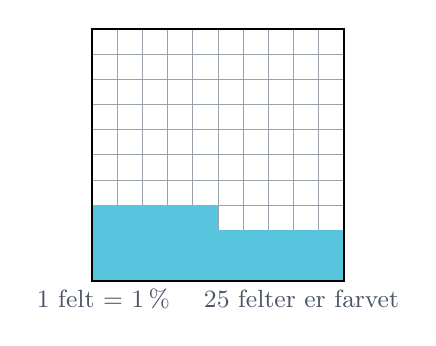
\begin{tikzpicture}[scale=0.32, line cap=round]
  \foreach \i in {0,...,9} \foreach \j in {0,...,9}
    \draw[line width=0.3pt, inksoft!55] (\i,\j) rectangle ++(1,1);
  \foreach \i in {0,...,9} \foreach \j in {0,...,1}
    \fill[accent] (\i,\j) rectangle ++(1,1);
  \foreach \i in {0,...,4} \fill[accent] (\i,2) rectangle ++(1,1);
  \draw[thick] (0,0) rectangle (10,10);
  \node[font=\small, text=inksoft] at (5,-0.7) {1 felt = 1\,\% \quad 25 felter er farvet};
\end{tikzpicture}
\end{center}

\begin{align*}
  1\,\% \text{ af } 480\,\text{kr} &= 4{,}8\,\text{kr}\\
  25 \cdot 4{,}8 &= 120\,\text{kr}\\[2pt]
  \Rightarrow\quad 25\,\% \text{ af } 480\,\text{kr} &= 120\,\text{kr}
\end{align*}

\begin{opgavebox}
\textbf{Opgave 2.1} \quad Hvad er $18\,\%$ af $450\,\text{kr}$?
\end{opgavebox}

\subsection*{Regel 2 --- Når prisen ændrer sig}

\begin{regelbox}
\textbf{Regel:} Stiger prisen med $p\,\%$, ganger du med $(1 + p/100)$. Falder
den med $p\,\%$, ganger du med $(1 - p/100)$. Husk: det er den \emph{nye}
pris, du ganger med.
\end{regelbox}

\textbf{Eksempel: En cykel kostede $2\,400\,\text{kr}$ og er nu $20\,\%$ billigere.}
\begin{align*}
  20\,\% \text{ af } 2\,400 &= 480\,\text{kr}\\
  2\,400 - 480 &= 1\,920\,\text{kr}\\[2pt]
  \text{Tjek: } 1\,920 \div 2\,400 &= 0{,}8 \quad\checkmark
\end{align*}

\begin{opgavebox}
\textbf{Opgave 2.2} \quad En jakke kostede $850\,\text{kr}$. Prisen stiger
$10\,\%$. Hvad koster jakken nu?
\end{opgavebox}

\begin{opgavebox}
\textbf{Opgave 2.3} \quad Prisen stiger $10\,\%$ og falder så igen $10\,\%$.
Prisen var $100\,\text{kr}$ til at starte med. Hvad er den nu? \hfill
{\small\color{inksoft}(Tænk dig om: er den $100\,\text{kr}$ igen?)}
\end{opgavebox}

\begin{opgavebox}
\textbf{Opgave 2.4} \quad $40\,\%$ af en klasse på $30$ elever har cykel.
Hvor mange elever har cykel?
\end{opgavebox}

\begin{opgavebox}
\textbf{Opgave 2.5} \quad En cykel kostede $400\,\text{kr}$ og kostede
senere $460\,\text{kr}$. Hvor stor er stigningen i procent? \hfill
{\small\color{inksoft}(Find først stigningen i kroner.)}
\end{opgavebox}

% ═════════════════════════════════════════════════════════════════════════════
\section{Sandsynlighed}
% ═════════════════════════════════════════════════════════════════════════════

\kompetence{Problembehandling}\kompetence{Ræsonnement}\kompetence{Repræsentation}

\noindent
Sandsynlighed (chance) fortæller, hvor stor en mulighed er. Vi skriver den
som en brøk: antal \emph{gunstige} udfald divideret med antal \emph{mulige}
udfald.

\begin{regelbox}
\textbf{Regel:} $\text{chance} = \dfrac{\text{gunstige udfald}}{\text{mulige
udfald}}$. Og summen af alle chancer i ét forsøg er $1$ (altså $100\,\%$).
Hvis du kaster to gange, er der $6 \cdot 6 = 36$ mulige udfald --- ikke $12$.
\end{regelbox}

\textbf{Eksempel: Kast en terning. Hvad er chancen for at få en 5'er?}

\begin{center}
\die{5} \qquad \text{\color{inksoft}(6 sider, 1 gavner)}
\end{center}

\begin{align*}
  \text{chance} &= \tfrac{1}{6} = 0{,}167 \approx 16{,}7\,\%\\[2pt]
  \text{Tjek: } \tfrac{1}{6}+\tfrac{1}{6}+\tfrac{1}{6}
    +\tfrac{1}{6}+\tfrac{1}{6}+\tfrac{1}{6} &= 1 \quad\checkmark
\end{align*}

\subsection*{Opgave 3.1 --- Én terning}

\begin{opgavebox}
\textbf{Opgave 3.1} \quad Du kaster én terning. Hvad er chancen for at få
et tal større end $4$?
\end{opgavebox}

\subsection*{Opgave 3.2 --- To terninger}

\begin{opgavebox}
\textbf{Opgave 3.2} \quad Du kaster to terninger. Hvad er chancen for at få
to ens tal?
\end{opgavebox}

\subsection*{Opgave 3.3 --- Krukken}

\noindent
I en krukke ligger $5$ røde, $3$ blå og $2$ grønne kugler. Du trækker én
kugle (uden at se).

\begin{center}
\krukke
\end{center}

\begin{opgavebox}
\textbf{Opgave 3.3} \quad Hvad er chancen for at trække en grøn kugle? Skriv
svaret som brøk, decimaltal og procent.
\end{opgavebox}

\subsection*{Opgave 3.4 --- Kortspillet}

\begin{opgavebox}
\textbf{Opgave 3.4} \quad Du trækker ét kort fra et almindeligt kortspil med
$32$ kort ($4$ farver $\times$ $8$ kort). Hvad er chancen for at få en hjerter?
\end{opgavebox}

\subsection*{Opgave 3.5 --- To mønter}

\begin{opgavebox}
\textbf{Opgave 3.5} \quad Du kaster en mønt to gange. Hvad er chancen for at
få \emph{mindst én} hjertes? \hfill
{\small\color{inksoft}(Tænk på den anden vej: hvad er chancen for at få
\textbf{to} kroner?)}
\end{opgavebox}

\subsection*{Opgave 3.6 --- Lottogitteret}

\noindent
Et lottogitter har $36$ felter ($6 \times 6$), og $4$ felter er markeret.

\begin{center}
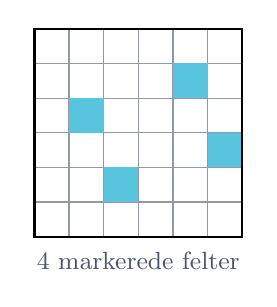
\begin{tikzpicture}[scale=0.44, line cap=round]
  \foreach \i in {0,...,5} \foreach \j in {0,...,5}
    \draw[line width=0.4pt, inksoft!60] (\i,\j) rectangle ++(1,1);
  \fill[accent] (1,3) rectangle ++(1,1);
  \fill[accent] (4,4) rectangle ++(1,1);
  \fill[accent] (2,1) rectangle ++(1,1);
  \fill[accent] (5,2) rectangle ++(1,1);
  \draw[thick] (0,0) rectangle (6,6);
  \node[font=\small, text=inksoft] at (3,-0.7) {4 markerede felter};
\end{tikzpicture}
\end{center}

\begin{opgavebox}
\textbf{Opgave 3.6} \quad Du rammer tilfældigt ét felt i gitteret. Hvad er
chancen for at ramme et markeret felt?
\end{opgavebox}

% ═════════════════════════════════════════════════════════════════════════════
\section{Trigonometri --- retvinklede trekanter}
% ═════════════════════════════════════════════════════════════════════════════

\kompetence{Problembehandling}\kompetence{Ræsonnement}\kompetence{Hjælpemidler}

\noindent
I en retvinklet trekant med vinkel $A$, hosliggende katete $b$, modstående
katete $a$ og hypotenuse $c$:

\vspace{6pt}
\begin{center}
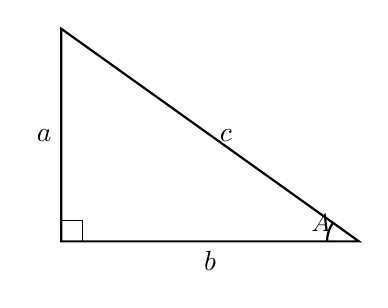
\begin{tikzpicture}[scale=0.9]
  \coordinate (B) at (0,0);
  \coordinate (A) at (4.2,0);
  \coordinate (C) at (0,3);
  \draw[thick] (B) -- (A) -- (C) -- cycle;
  \draw ($(B)+(0.30,0)$) -- ($(B)+(0.30,0.30)$) -- ($(B)+(0,0.30)$);
  \draw[thick] ($(A)+(180:0.45)$) arc[start angle=180, end angle=144.5, radius=0.45];
  \node[anchor=west] at ($(A)+(162:0.85)$) {\small $A$};
  \path (B) -- node[below] {$b$} (A);
  \path (A) -- node[right] {$c$} (C);
  \path (B) -- node[left]  {$a$} (C);
\end{tikzpicture}
\qquad
$\cos(A) = \dfrac{b}{c} \qquad
 \sin(A) = \dfrac{a}{c} \qquad
 \tan(A) = \dfrac{a}{b}$
\end{center}

\begin{regelbox}
\textbf{Regel:} Pythagoras siger $a^{2} + b^{2} = c^{2}$. Skal du finde en
katete, isolerer du først --- så kvadratroden til sidst. Skal du finde en
vinkel, så finder du et forhold (sin, cos eller tan) og bruger lommeregnerens
$\sin^{-1}$, $\cos^{-1}$ eller $\tan^{-1}$.
\end{regelbox}

\textbf{Eksempel: $a = 5\,\text{cm}$, $c = 13\,\text{cm}$. Find $A$.}

\begin{align*}
  \sin(A) &= \tfrac{a}{c} = \tfrac{5}{13} = 0{,}385\\
  A &= \sin^{-1}(0{,}385) \approx 22{,}6^{\circ}
\end{align*}
Tjek: $\cos(A) = \tfrac{12}{13}$, og $\sin^{2}A + \cos^{2}A = 1$ \checkmark

\subsection*{Opgave 4.1 --- Find hypotenusen}

\begin{opgavebox}
\textbf{Opgave 4.1} \quad I en retvinklet trekant er kateterne $9\,\text{cm}$
og $12\,\text{cm}$. Find hypotenusen $c$.
\end{opgavebox}

\subsection*{Opgave 4.2 --- Find den manglende katete}

\begin{opgavebox}
\textbf{Opgave 4.2} \quad Hypotenusen er $c = 13\,\text{cm}$ og den hosliggende
katete er $b = 5\,\text{cm}$. Find den modstående katete $a$.
\end{opgavebox}

\subsection*{Opgave 4.3 --- Find vinklen}

\begin{opgavebox}
\textbf{Opgave 4.3} \quad Den modstående katete er $a = 7\,\text{cm}$ og
hypotenusen er $c = 15\,\text{cm}$. Find vinklen $A$.
\end{opgavebox}

\subsection*{Opgave 4.4 --- Stigen mod muren}

\noindent
En stige på $6\,\text{m}$ læner mod en mur. Vinklen mod jorden er $60^{\circ}$.

\begin{center}
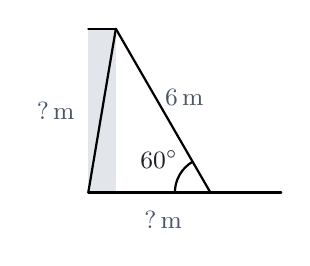
\begin{tikzpicture}[scale=1.0, line cap=round, line join=round]
  \fill[graysk] (0,0) rectangle (0.35,2.078);
  \draw[thick] (0,0) -- (0.35,2.078);
  \draw[thick] (0,2.078) -- (0.35,2.078);
  \draw[thick] (0.35,2.078) -- (1.55,0);
  \draw[thick] (0,0) -- (2.45,0);
  \draw[thick] (1.55,0) ++(180:0.45) arc[start angle=180, end angle=120, radius=0.45];
  \node[font=\small, text=ink] at (0.90,0.42) {$60^{\circ}$};
  \node[font=\small, text=inksoft] at (1.22,1.20) {$6\,\text{m}$};
  \node[below, font=\small, text=inksoft] at (0.95,-0.12) {$?\,\text{m}$};
  \node[left, font=\small, text=inksoft] at (-0.05,1.04) {$?\,\text{m}$};
\end{tikzpicture}
\end{center}

\begin{opgavebox}
\textbf{Opgave 4.4} \quad Hvor høj er muren? Og hvor langt er stagens fod fra
murens base? \hfill
{\small\color{inksoft}(Brug $\sin$ og $\cos$ på $60^{\circ}$.)}
\end{opgavebox}

\subsection*{Opgave 4.5 --- Bakken ned mod vandet}

\noindent
Du står oven på en bakke. Vandet ligger $30\,\text{m}$ under dine fødder, og
du ser vinklen $45^{\circ}$ ned til en båd i vandet.

\begin{center}
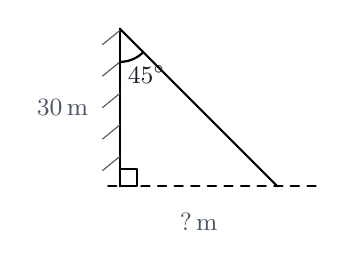
\begin{tikzpicture}[scale=1.0, line cap=round, line join=round]
  \draw[thick] (0,0) -- (0,2.0);
  \foreach \y in {0.2,0.6,1.0,1.4,1.8}
    \draw[thin, inksoft] (-0.22,\y) -- (0,\y+0.18);
  \draw[thick] (0,2.0) -- (2.0,0);
  \draw[thick, dashed] (-0.15,0) -- (2.55,0);
  \draw[thick] (0,0) -- (0.22,0) -- (0.22,0.22) -- (0,0.22);
  \draw[thick] (0,2.0) ++(270:0.42) arc[start angle=270, end angle=315, radius=0.42];
  \node[font=\small, text=ink] at (0.34,1.42) {$45^{\circ}$};
  \node[left, font=\small, text=inksoft] at (-0.28,1.0) {$30\,\text{m}$};
  \node[below, font=\small, text=inksoft] at (1.0,-0.22) {$?\,\text{m}$};
\end{tikzpicture}
\end{center}

\begin{opgavebox}
\textbf{Opgave 4.5} \quad Hvor langt er der fra bakken (lodret ned) til båden?
\end{opgavebox}

% ═════════════════════════════════════════════════════════════════════════════
\section{2D-geometri --- areal og omkreds}
% ═════════════════════════════════════════════════════════════════════════════

\kompetence{Problembehandling}\kompetence{Modellering}\kompetence{Repræsentation}

\noindent
Areal er fladens størrelse (målt i $\text{cm}^{2}$), omkreds er længen rundt
om (målt i $\text{cm}$). Husk: $\pi \approx 3{,}14$.

\begin{regelbox}
\textbf{Regel:} \quad
Trekant: $\text{areal} = \tfrac{b \cdot h}{2}$ \quad
Rektangel: $\text{areal} = l \cdot b$, \quad $\text{omkreds} = 2l + 2b$ \quad
Cirkel: $\text{areal} = \pi r^{2}$, \quad $\text{omkreds} = 2\pi r$
\end{regelbox}

\textbf{Eksempel: Trekant med grundlinje $14\,\text{cm}$ og højde $9\,\text{cm}$}
\begin{align*}
  \text{areal} &= \tfrac{b \cdot h}{2}
                = \tfrac{14 \cdot 9}{2}
                = \tfrac{126}{2}
                = 63\,\text{cm}^{2}
\end{align*}

\subsection*{Opgave 5.1 --- Rektanglet}

\begin{opgavebox}
\textbf{Opgave 5.1} \quad Et rektangel er $12\,\text{cm}$ langt og
$7\,\text{cm}$ bredt. Find arealet og omkredsen.
\end{opgavebox}

\subsection*{Opgave 5.2 --- Trekanten}

\begin{opgavebox}
\textbf{Opgave 5.2} \quad En trekant har grundlinje $16\,\text{cm}$ og højde
$9\,\text{cm}$. Find arealet.
\end{opgavebox}

\subsection*{Opgave 5.3 --- Cirklen}

\begin{opgavebox}
\textbf{Opgave 5.3} \quad En cirkel har radius $6\,\text{cm}$. Find omkredsen
og arealet. \hfill {\small\color{inksoft}(Brug $\pi \approx 3{,}14$.)}
\end{opgavebox}

\subsection*{Opgave 5.4 --- Sammensat figur}

\noindent
Figuren består af et rektangel ($12\,\text{cm} \times 6\,\text{cm}$) med en
halvcircle ovenpå. Halvcirklens diameter er $6\,\text{cm}$, så radius er
$3\,\text{cm}$.

\begin{center}
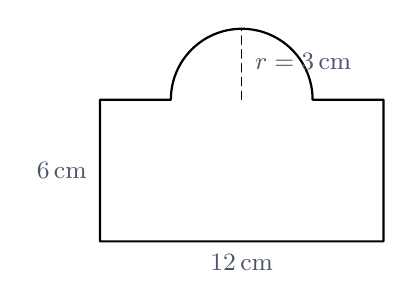
\begin{tikzpicture}[scale=0.30, line cap=round, line join=round]
  \draw[thick] (0,0) -- (12,0) -- (12,6) -- (9,6) arc[start angle=0, end angle=180, radius=3] -- (3,6) -- (0,6) -- cycle;
  \draw[densely dashed, line width=0.5pt] (6,6) -- (6,9);
  \node[right, font=\small, text=inksoft] at (6.15,7.6) {$r = 3\,\text{cm}$};
  \node[below, font=\small, text=inksoft] at (6,-0.12) {$12\,\text{cm}$};
  \node[left, font=\small, text=inksoft] at (-0.15,3) {$6\,\text{cm}$};
\end{tikzpicture}
\end{center}

\begin{opgavebox}
\textbf{Opgave 5.4} \quad Find arealet og omkredsen af hele figuren.
\end{opgavebox}

\subsection*{Opgave 5.5 --- Stigen i haven}

\begin{opgavebox}
\textbf{Opgave 5.5} \quad En stige er $5\,\text{m}$ lang og når $4\,\text{m}$
op ad en mur. Hvor langt er der fra stagens fod til murens base? \hfill
{\small\color{inksoft}(Brug Pythagoras.)}
\end{opgavebox}

% ═════════════════════════════════════════════════════════════════════════════
\section{3D-geometri --- rumfang og overflade}
% ═════════════════════════════════════════════════════════════════════════════

\kompetence{Problembehandling}\kompetence{Modellering}\kompetence{Repræsentation}

\noindent
Rumfang er pladsen inde i figuren (målt i $\text{cm}^{3}$), overfladeareal er
summen af alle fladerne (målt i $\text{cm}^{2}$). Husk for kassen:
overfladen er $6$ flader, ikke $3$ --- og der er $2$ af hver slags.

\begin{regelbox}
\textbf{Regel:} \quad
Kasse: $\text{rumfang} = l \cdot b \cdot h$, \quad
$\text{overflade} = 2(lb + lh + bh)$ \\[3pt]
Cylinder: $\text{rumfang} = \pi r^{2} h$, \quad
$\text{overflade} = 2\pi r^{2} + 2\pi r h$
\end{regelbox}

\textbf{Eksempel: Kasse $12\,\text{cm} \times 8\,\text{cm} \times 5\,\text{cm}$}

\begin{center}
\kassefigur{$12\,\text{cm}$}{$8\,\text{cm}$}{$5\,\text{cm}$}{0.95}
\end{center}

\begin{align*}
  \text{rumfang} &= 12 \cdot 8 \cdot 5 = 480\,\text{cm}^{3}\\[3pt]
  \text{overflade} &= 2(12\cdot 8 + 12\cdot 5 + 8\cdot 5)\\
                   &= 2(96 + 60 + 40) = 2 \cdot 196 = 392\,\text{cm}^{2}
\end{align*}

\subsection*{Opgave 6.1 --- En anden kasse}

\begin{opgavebox}
\textbf{Opgave 6.1} \quad En kasse er $10\,\text{cm} \times 6\,\text{cm}
\times 4\,\text{cm}$. Find rumfanget og overfladearealet.
\end{opgavebox}

\subsection*{Opgave 6.2 --- Cylinderen}

\begin{center}
\cylinderfigur{$r = 5\,\text{cm}$}{$h = 12\,\text{cm}$}{0.95}
\end{center}

\begin{opgavebox}
\textbf{Opgave 6.2} \quad Find cylinderens rumfang og overfladeareal.
\hfill {\small\color{inksoft}(Brug $\pi \approx 3{,}14$.)}
\end{opgavebox}

\subsection*{Opgave 6.3 --- Hvad fylder mest?}

\begin{opgavebox}
\textbf{Opgave 6.3} \quad En kasse er $20\,\text{cm} \times 20\,\text{cm}
\times 20\,\text{cm}$. En cylinder har $r = 8\,\text{cm}$ og $h = 16\,\text{cm}$.
Hvilken af de to fylder mest? \hfill
{\small\color{inksoft}(Svar i liter: $1\,\text{L} = 1\,000\,\text{cm}^{3}$.)}
\end{opgavebox}

\subsection*{Opgave 6.4 --- Overfladen af en cylinder}

\begin{opgavebox}
\textbf{Opgave 6.4} \quad En cylinder har $r = 3\,\text{cm}$ og
$h = 10\,\text{cm}$. Find overfladearealet. \hfill
{\small\color{inksoft}(Der er to flader med cirkel og to med side.)}
\end{opgavebox}

\subsection*{Opgave 6.5 --- Vandbeholderen}

\begin{opgavebox}
\textbf{Opgave 6.5} \quad En vandbeholder er en kasse med bund
$25\,\text{cm} \times 20\,\text{cm}$. Den skal rumme $1$ liter vand. Hvor høj
skal den være?
\end{opgavebox}

% ═════════════════════════════════════════════════════════════════════════════
\newpage
\section*{Appendix --- Facit}
% ═════════════════════════════════════════════════════════════════════════════

\begin{multicols}{2}
\small
\setlength{\parindent}{0pt}

\noindent\textbf{Brøker}
\begin{itemize}[leftmargin=1.3em, itemsep=1pt, topsep=2pt]
  \item \textbf{1.1:} $63 \div 7 = 9$, og $2 \cdot 9 = 18$
  \item \textbf{1.2:} $32 \div 8 = 4$, og $3 \cdot 4 = 12$ elever
  \item \textbf{1.3:} $0{,}45 = \tfrac{45}{100} = \tfrac{9}{20}$
  \item \textbf{1.4:} $\tfrac{2}{5} = 0{,}4 = 40\,\%$
  \item \textbf{1.5:} Fællesnævner $15$: $\tfrac{2}{3} = \tfrac{10}{15}$ og
        $\tfrac{3}{5} = \tfrac{9}{15}$. $10 > 9$, så $\tfrac{2}{3}$ er størst
\end{itemize}

\noindent\textbf{Procentregning}
\begin{itemize}[leftmargin=1.3em, itemsep=1pt, topsep=2pt]
  \item \textbf{2.1:} $18\,\%$ af $450$: $4{,}5 \cdot 18 = 81\,\text{kr}$
  \item \textbf{2.2:} $10\,\%$ af $850 = 85$, så $850 + 85 = 935\,\text{kr}$
  \item \textbf{2.3:} $100 \cdot 1{,}1 = 110$, og $110 \cdot 0{,}9 = 99\,\text{kr}$.
        Prisen er $1\,\%$ lavere end til at starte med
  \item \textbf{2.4:} $40\,\%$ af $30 = 12$ elever
  \item \textbf{2.5:} Stigning $460 - 400 = 60\,\text{kr}$, og
        $60 \div 400 = 0{,}15 = 15\,\%$
\end{itemize}

\noindent\textbf{Sandsynlighed}
\begin{itemize}[leftmargin=1.3em, itemsep=1pt, topsep=2pt]
  \item \textbf{3.1:} $2$ af $6$ sider: $\tfrac{2}{6} = \tfrac{1}{3} \approx 33{,}3\,\%$
  \item \textbf{3.2:} $6$ kast ($1$-$1$, $2$-$2$, ...) ud af $36$:
        $\tfrac{6}{36} = \tfrac{1}{6} \approx 16{,}7\,\%$
  \item \textbf{3.3:} $2$ grønne ud af $10$: $\tfrac{2}{10} = \tfrac{1}{5} = 0{,}2 = 20\,\%$
  \item \textbf{3.4:} $8$ hjerter ud af $32$: $\tfrac{8}{32} = \tfrac{1}{4} = 25\,\%$
  \item \textbf{3.5:} To kroner: $\tfrac{1}{2}\cdot\tfrac{1}{2} = \tfrac{1}{4}$.
        Så chance for mindst én hjertes $= 1 - \tfrac{1}{4} = \tfrac{3}{4} = 75\,\%$
  \item \textbf{3.6:} $4$ markerede ud af $36$: $\tfrac{4}{36} = \tfrac{1}{9} \approx 11{,}1\,\%$
\end{itemize}

\columnbreak

\noindent\textbf{Trigonometri}
\begin{itemize}[leftmargin=1.3em, itemsep=1pt, topsep=2pt]
  \item \textbf{4.1:} $c^{2} = 9^{2} + 12^{2} = 81 + 144 = 225 \Rightarrow c = 15\,\text{cm}$
  \item \textbf{4.2:} $a^{2} = 13^{2} - 5^{2} = 169 - 25 = 144 \Rightarrow a = 12\,\text{cm}$
  \item \textbf{4.3:} $\sin A = \tfrac{7}{15} = 0{,}4667 \Rightarrow A \approx 27{,}8^{\circ}$
  \item \textbf{4.4:} $h = 6 \cdot \sin 60^{\circ} = 6 \cdot 0{,}866 = 5{,}20\,\text{m}$;
        $d = 6 \cdot \cos 60^{\circ} = 6 \cdot 0{,}5 = 3{,}00\,\text{m}$
  \item \textbf{4.5:} $\tan 45^{\circ} = \tfrac{30}{x} \Rightarrow 1 = \tfrac{30}{x}
        \Rightarrow x = 30\,\text{m}$
\end{itemize}

\noindent\textbf{2D-geometri}
\begin{itemize}[leftmargin=1.3em, itemsep=1pt, topsep=2pt]
  \item \textbf{5.1:} Areal $12 \cdot 7 = 84\,\text{cm}^{2}$;
        omkreds $2 \cdot 12 + 2 \cdot 7 = 38\,\text{cm}$
  \item \textbf{5.2:} $\tfrac{16 \cdot 9}{2} = 72\,\text{cm}^{2}$
  \item \textbf{5.3:} Omkreds $2 \cdot 3{,}14 \cdot 6 = 37{,}68\,\text{cm}$;
        areal $3{,}14 \cdot 6^{2} = 113{,}04\,\text{cm}^{2}$
  \item \textbf{5.4:} Areal $12 \cdot 6 + \tfrac{1}{2}\pi \cdot 3^{2}
        = 72 + 14{,}13 = 86{,}13\,\text{cm}^{2}$;
        omkreds $12 + 6 + 6 + 3 + 3 + \pi \cdot 3 = 39{,}42\,\text{cm}$
        (de to $3\,\text{cm}$ er de vandrette topstykker)
  \item \textbf{5.5:} $\sqrt{5^{2} + 4^{2}} = \sqrt{41} \approx 6{,}40\,\text{m}$
\end{itemize}

\noindent\textbf{3D-geometri}
\begin{itemize}[leftmargin=1.3em, itemsep=1pt, topsep=2pt]
  \item \textbf{6.1:} Rumfang $10 \cdot 6 \cdot 4 = 240\,\text{cm}^{3}$;
        overflade $2(10\cdot 6 + 10\cdot 4 + 6\cdot 4)
        = 2(60 + 40 + 24) = 248\,\text{cm}^{2}$
  \item \textbf{6.2:} Rumfang $3{,}14 \cdot 5^{2} \cdot 12 = 942\,\text{cm}^{3}$;
        overflade $2\cdot 3{,}14 \cdot 5^{2} + 2\cdot 3{,}14 \cdot 5 \cdot 12
        = 157 + 376{,}8 = 533{,}8\,\text{cm}^{2}$
  \item \textbf{6.3:} Kasse $20^{3} = 8\,000\,\text{cm}^{3} = 8\,\text{L}$.
        Cylinder $3{,}14 \cdot 8^{2} \cdot 16 = 3\,215{,}4\,\text{cm}^{3}
        \approx 3{,}2\,\text{L}$. \textbf{Kassen fylder mest}
  \item \textbf{6.4:} $2 \cdot 3{,}14 \cdot 3^{2} + 2 \cdot 3{,}14 \cdot 3 \cdot 10
        = 56{,}52 + 188{,}4 = 244{,}92\,\text{cm}^{2}$
  \item \textbf{6.5:} $1\,\text{L} = 1\,000\,\text{cm}^{3}$, og
        $1\,000 \div (25 \cdot 20) = 1\,000 \div 500 = 2\,\text{cm}$
\end{itemize}

\end{multicols}

\end{document}
